\documentclass[10pt]{article}
\usepackage{kdnotes}
\usepackage{multicol}
\usepackage{tikz}

\usetikzlibrary{shapes} 

\tikzset{
subtree/.style={
	  draw,shape border uses incircle,
	    isosceles triangle,shape border rotate=90,yshift=-0.9cm, minimum
    height=8mm}
}


\newcommand{\node}{\texttt{node}}
\usepackage{verbatim}
\begin{document}
\title{Some topics in Algorithms}
\author{Working draft}
\maketitle
\hrule
\begin{multicols}{2}
{\footnotesize \tableofcontents }
\end{multicols}
\hrule

\section{Red-Black Trees}
\begin{center}
\fbox{
\begin{minipage}{0.8\textwidth}
{\sf Main aim of this write up is to answer why are the operations of RB
	tree defined the way they are, why are the cases considered exhaustive
	etc. So there could be more cases than what may be present in standard
	texts like CLRS. They are included here solely for pedagogic/clarity
	purpose. Note added : Thanks to Gautam for comments.} 
\end{minipage}
}
\end{center}
Red-Back tree (RB tree) is a binary search tree with the following extra
invariants.  
\begin{definition}{Invariants of Red-back trees}
\begin{enumerate}
	\item Each node of a RB-tree must be colored red (R) or black (B).
		\label{r_or_b}
	\item Root node must be black. \label{r_m_b}
	\item A red node must have two black children. \label{r_m_bc}
	\item The number of black nodes from a given node to all of its 
		leaves must be the same (along all paths). \label{bh}
\end{enumerate}
\end{definition}
Leaf nodes of RB tree has special sentinel nodes which are colored black as
their children. We will denote sentinel nodes by squares and non-sentinel
nodes by circle in diagrams.

\begin{definition}
For a node $x$ in the RB tree, we call the number of black nodes counted
excluding $x$ for any path starting from $x$ to a leaf as the \emph{black
height} of $x$ (denoted as $bh(x)$).
\end{definition}
Since every path from a node to leaf must be of same length by
property~\ref{bh}, this quantity is well defined. Black height of a sentinel
node is zero. Due to this sentinel nodes, black height of every non-sentinel
node must be at least $1$. Black height of a RB-tree is the black
height of the root of the tree.

Why are the properties of RB tree interesting ? They are important as they
help in ensuring that the resulting tree formed is balanced i,e. has height
$O(\log n)$ where $n$ is the number of nodes. A proof can be found in CLRS.
\begin{lemma}
Height of red black tree of $n$ nodes is at most $2\log (n+1)$
\end{lemma}

The above lemma shows that in order to ensure that we get an $O(\log n)$ depth
tree, it suffices to ensure that we design insert and delete procedures such
that all these properties of RB tree are guaranteed to holds.

In the subsequent sections we explain how insertion and deletion can be
designed to achieve this.

\subsection{Main Idea in Insertion}
The main idea is to perform a binary search traversal of the tree and insert
the node as a leaf in the location found. We then color the node red. Now we
need to ensure that the four properties still hold. If any violation of the
properties occur, we need to make suitable modifications so that these
properties are restored.

Following are the steps taken while inserting a node.
\begin{enumerate}
\item Insert at appropriate leaf location after performing a binary search
traversal.
\item Colour the new node red.
\item Call {\tt RB-Tree-Fixup} procedure on this node.
\end{enumerate}

\subsection{Fixing the violations in RB-tree after Tree insert}
In this section, we explain how any violation of the four RB tree properties
 can be fixed.

Let $x$ denote the newly inserted node. We use $p(x)$ to denote
the parent of the node and $c(x)$ to denote a child (subscripts will be
used to differentiate the left and right child). 

Let us first consider the base cases. If $p(x)$ does not exists, then
the node must be the root node. We can observe that only the
property~\ref{r_m_b} is violated (as there can be no other nodes). So this can
be fixed by coloring $x$ black. Now, if $p(x)$ exists then we check if the
parent is colored black. If yes, we can observe that there are no violation
of the properties. If the parent of the $x$ is colored red, then there is
violation of property that red node must have black children 
(property~\ref{r_m_bc}) which, henceforth, we call as the `red-red
violation'. This needs to be fixed. To summarise, following is a ``C'' style
pseudo code of what is done so far.

\begin{verbatim}
RB-Tree-Fixup(Node* node)
{
        if(node->parent == NULL){        // node is root
                node->colour = BLACK;
                return 0;
        }
        else if(node->parent->colour == BLACK)
                return 0; // No violation.
        else
                return fixup-Uncle-Red(node);
}
\end{verbatim}
In the rest of the section, we explain what are the major cases that arise
while we fix the red-red violation. We also show that while fixing the red-red
violation all other invariants are maintained.

Let us first analyse the current situation and see what could possibly be done
to handle the violation. We assume that the tree that we have in hand is a
valid RB tree except for this red-red violation.

Let $x$ be the node to be deleted. We know that the color of $x$ and $p(x)$ 
are both red. The current situation is as shown in this diagram.
\begin{center}
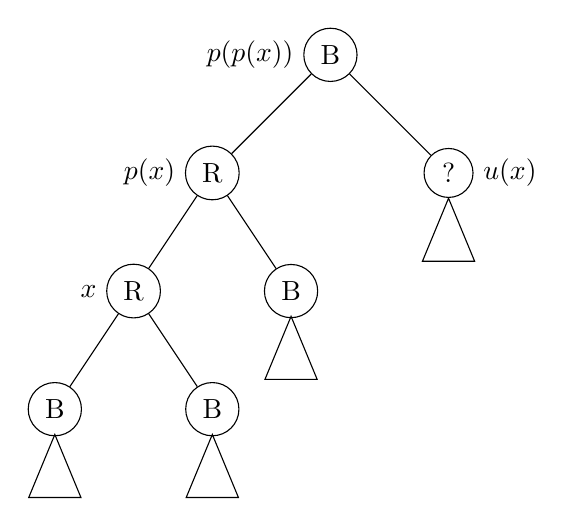
\begin{tikzpicture}[sibling distance=3cm, level 2/.style={sibling distance
	=2cm}]
	\node[draw, circle, label=west:$p(p(x))$] {B}
	child{ node[circle, draw, label=west:$p(x)$] {R} 
		child { node[circle, draw, label=west:$x$] {R}
			child { node[circle, draw] {B} { node[subtree] {} }}
			child { node[circle, draw] {B} { node[subtree] {} }}
		}
		child { node[circle, draw] {B} { node[subtree] {} }}
	}
	child{ node[circle, draw, label=east:$u(x)$] {?} { node[subtree] {} }};
\end{tikzpicture}
\end{center}
One might ask why should there be a grand parent for $x$ (i,e. parent of
parent of $x$). The reason is that the tree must have a root and
$p(x)$ cannot be a root as root should be black (property~\ref{r_m_b}). Hence
$p(x)$ must have a parent. Also $p(p(x))$ cannot be red in color as $p(x)$ is
red (Here we are using the fact that we had a proper RB tree when we started).
Hence $p(p(x))$ must be black. Note that children of $x$ must be black as $x$
is red (property~\ref{r_m_bc}). We do not know the color of right child of
$p(p(x))$. So we need to consider the various possibilities and see how to fix
the red-red violation. The triangles below a node shows a subtree rooted at
that node. Note that the subtree could also be empty (i,e. children of $x$
could also be just sentinels).

For convenience call the right child of $p(p(x))$ as \emph{uncle of $x$}
denoted as $u(x)$. Clearly, there will be two cases : one where $u(x)$ is red,
other where $u(x)$ is black. 

\begin{remark}
In each of the cases that follows, we first explain the most general sub case
that arise and show how the remaining sub cases can be reduced to this main
case.
\end{remark}

\subsubsection{Uncle is red}
Let us assume that $x$ is a \emph{left child} of $p(x)$. We will
handle the case where $x$ is a right child of $p(x)$ later.

\fbox{{\bf $x$ is left child of $p(x)$ :}}
To remove the red-red violation, we do the following : color $p(x), u(x)$
black and $p(p(x))$ red. This can be thought of as ``pushing'' the black color
of $p(p(x))$ to its children. This causes the black height at $p(p(x))$
increase by $1$. Note that all other properties are satisfied except for the
fact that coloring $p(p(x))$ might result in a red-red violation at $p(p(x))$
if its parent is red. In that case, we call {\tt RB-Tree-Fixup()} at $p(p(x))$
(i,e. $p(p(x))$ will be the new $x$). Figure below shows the situation before
and after the transformation.

\begin{center}
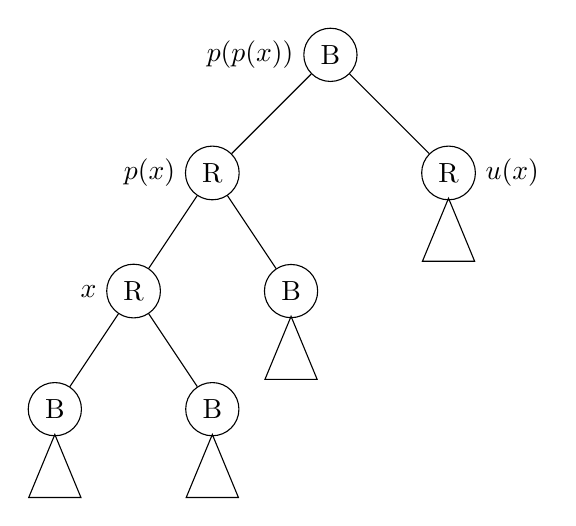
\begin{tikzpicture}[sibling distance=3cm, level 2/.style={sibling distance
	=2cm}]
	\node[draw, circle, label=west:$p(p(x))$] {B}
	child{ node[circle, draw, label=west:$p(x)$] {R} 
		child { node[circle, draw, label=west:$x$] {R}
			child { node[circle, draw] {B} { node[subtree] {} }}
			child { node[circle, draw] {B} { node[subtree] {} }}
		}
		child { node[circle, draw] {B} { node[subtree] {} }}
	}
	child{ node[circle, draw, label=east:$u(x)$] {R} { node[subtree] {} }};
\end{tikzpicture} 
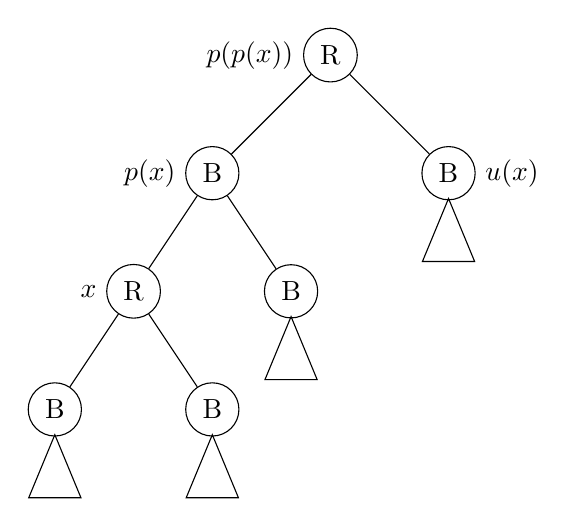
\begin{tikzpicture}[sibling distance=3cm, level 2/.style={sibling distance
	=2cm}]
	\node[draw, circle, label=west:$p(p(x))$] {R}
	child{ node[circle, draw, label=west:$p(x)$] {B} 
		child { node[circle, draw, label=west:$x$] {R}
			child { node[circle, draw] {B} { node[subtree] {} }}
			child { node[circle, draw] {B} { node[subtree] {} }}
		}
		child { node[circle, draw] {B} { node[subtree] {} }}
	}
	child{ node[circle, draw, label=east:$u(x)$] {B} { node[subtree] {} }};

\end{tikzpicture}
\end{center}

\fbox{{\bf $x$ is right child of $p(x)$ :}} In this case too the same
recoloring strategy works. 
\begin{center}
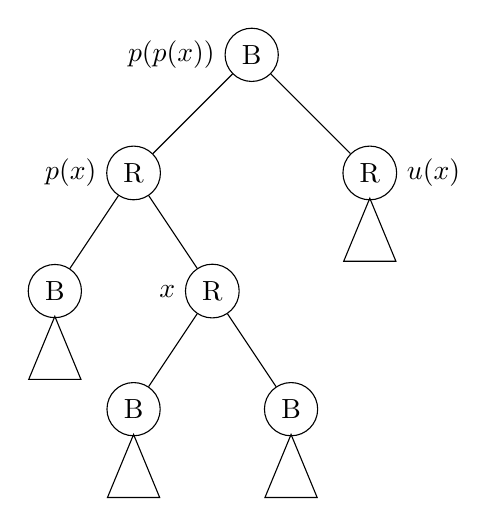
\begin{tikzpicture}[sibling distance=3cm, level 2/.style={sibling distance
	=2cm}]
	\node[draw, circle, label=west:$p(p(x))$] {B}
	child{ node[circle, draw, label=west:$p(x)$] {R} 
		child { node[circle, draw] {B} { node[subtree] {} }}
		child { node[circle, draw, label=west:$x$] {R}
			child { node[circle, draw] {B} { node[subtree] {} }}
			child { node[circle, draw] {B} { node[subtree] {} }}
		}
	}
	child{ node[circle, draw, label=east:$u(x)$] {R} { node[subtree] {} }};
\end{tikzpicture} \quad
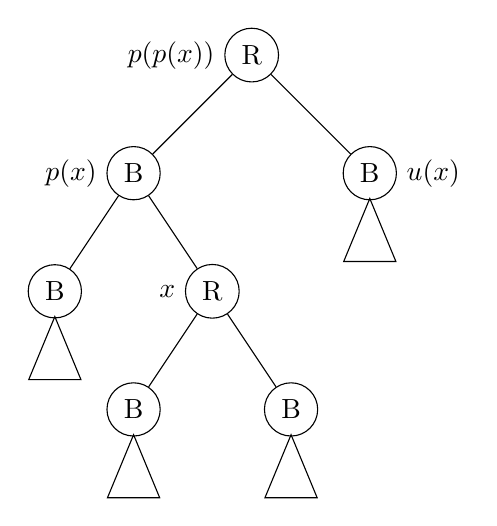
\begin{tikzpicture}[sibling distance=3cm, level 2/.style={sibling distance
	=2cm}]
	\node[draw, circle, label=west:$p(p(x))$] {R}
	child{ node[circle, draw, label=west:$p(x)$] {B} 
		child { node[circle, draw] {B} { node[subtree] {} }}
		child { node[circle, draw, label=west:$x$] {R}
			child { node[circle, draw] {B} { node[subtree] {} }}
			child { node[circle, draw] {B} { node[subtree] {} }}
		}
	}
	child{ node[circle, draw, label=east:$u(x)$] {B} { node[subtree] {} }};

\end{tikzpicture}
\end{center}
Pseudo code corresponding to the
case where uncle is red is as follows.
\begin{verbatim}
int fixup-Uncle-Red(Node* node)
{
        Node* gp = grandparent(node);
        Node* u  = uncle(node);

        if(u->colour == RED){
                node->parent->colour = BLACK;
                gp->colour = RED;
                u->colour = BLACK;
                RB-Tree-fixup(gp);
                return 1;
        }else
                return fixup-Uncle-black-spl(node);
}
\end{verbatim}

\subsubsection{Uncle is black}
Here also we have two cases with $x$ begin left, right child of $p(x)$.

\fbox{{\bf $x$ is left child of $p(x)$} :} The situation in this case is
shown. Here, we interchange the colors of $p(x)$ and $p(p(x))$ and get the
following. 

\begin{center}
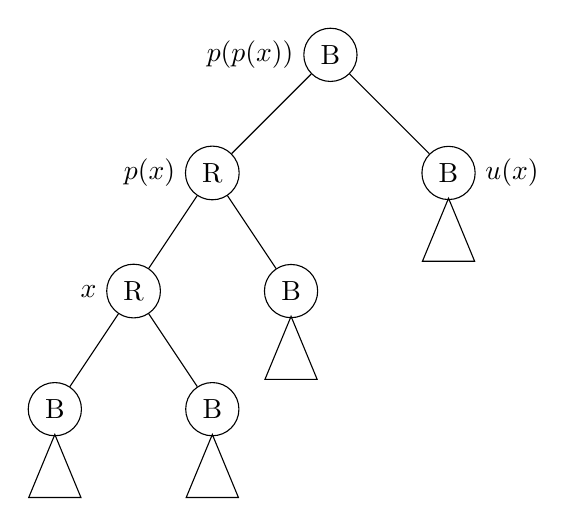
\begin{tikzpicture}[sibling distance=3cm, level 2/.style={sibling distance
	=2cm}]
	\node[draw, circle, label=west:$p(p(x))$] {B}
	child{ node[circle, draw, label=west:$p(x)$] {R} 
		child { node[circle, draw, label=west:$x$] {R}
			child { node[circle, draw] {B} { node[subtree] {} }}
			child { node[circle, draw] {B} { node[subtree] {} }}
		}
		child { node[circle, draw] {B} { node[subtree] {} }}
	}
	child{ node[circle, draw, label=east:$u(x)$] {B} { node[subtree] {} }};
\end{tikzpicture} 
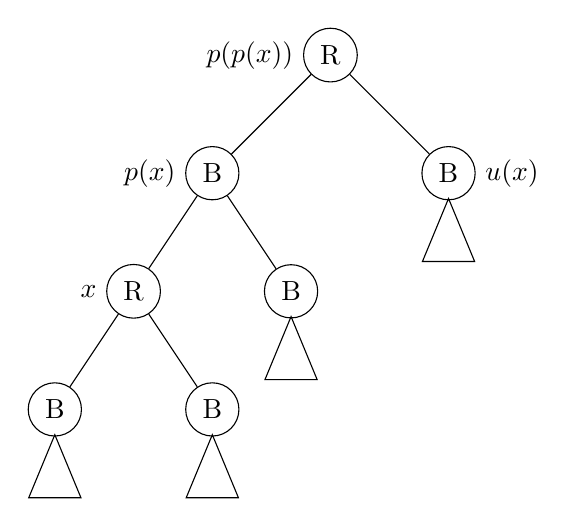
\begin{tikzpicture}[sibling distance=3cm, level 2/.style={sibling distance
	=2cm}]
	\node[draw, circle, label=west:$p(p(x))$] {R}
	child{ node[circle, draw, label=west:$p(x)$] {B} 
		child { node[circle, draw, label=west:$x$] {R}
			child { node[circle, draw] {B} { node[subtree] {} }}
			child { node[circle, draw] {B} { node[subtree] {} }}
		}
		child { node[circle, draw] {B} { node[subtree] {} }}
	}
	child{ node[circle, draw, label=east:$u(x)$] {B} { node[subtree] {} }};

\end{tikzpicture}
\end{center}

With this interchange, black height along the left child of
$p(p(x))$ has increased by $1$ while along the right remained the same. So to
balance out, we perform a rotation of $p(p(x))$ around $p(x)$ (i,e. right
rotate of $p(p(x))$).

\begin{center}
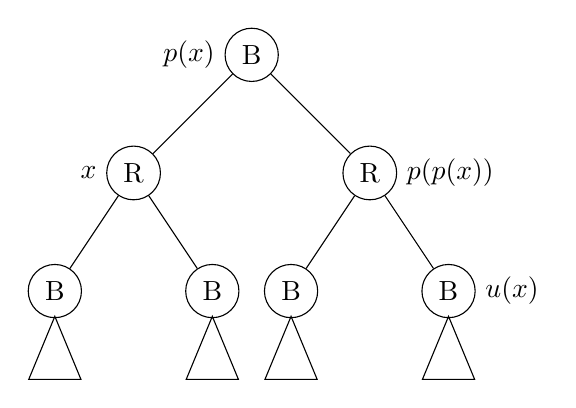
\begin{tikzpicture}[sibling distance=3cm, level 2/.style={sibling distance
	=2cm}]
	\node[draw, circle, label=west:$p(x)$] {B}
	child{ node[circle, draw, label=west:$x$] {R} 
		child { node[circle, draw] {B} { node[subtree] {} }}
		child { node[circle, draw] {B} { node[subtree] {} }}
	}
	child{ node[circle, draw, label=east:$p(p(x))$] {R} 
		child { node[circle, draw] {B} { node[subtree] {} }}
		child { node[circle, draw, label=east:$u(x)$] {B} { node[subtree] {} }}
	};
\end{tikzpicture}
\end{center}
Now note that there is no more red-red violation and right rotation fixes
the black height. Since there are no more violations we can stop here.

\fbox{{\bf $x$ is right child of $p(x)$ :}} 
Our aim is to reduce this case to the previous case where $x$ is the left
child $p(x)$.  Before giving the details, note in the earlier that we
crucially used the fact that $p(x)$ is the left child of $p(p(x))$. Hence we
need to consider the cases where $p(x)$ is a left, right child of $p(p(x))$.
%(Note that this was not necessary in the earlier case as we did not need to
%perform any rotation involving $p(p(x))$.)

{\bf Sub case 1 -- $p(x)$ is left child of $p(p(x))$ :} Note that uncle of $x$
will be black. 
\begin{center}
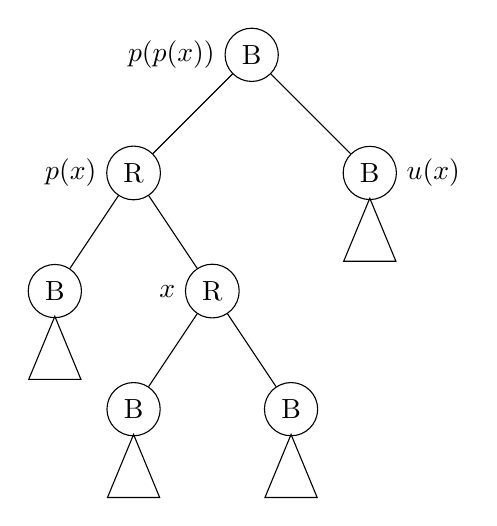
\begin{tikzpicture}[sibling distance=3cm, level 2/.style={sibling distance
	=2cm}]
	\node[draw, circle, label=west:$p(p(x))$] {B}
	child{ node[circle, draw, label=west:$p(x)$] {R} 
		child { node[circle, draw] {B} { node[subtree] {} }}
		child { node[circle, draw, label=west:$x$] {R}
			child { node[circle, draw] {B} { node[subtree] {} }}
			child { node[circle, draw] {B} { node[subtree] {} }}
		}
	}
	child{ node[circle, draw, label=east:$u(x)$] {B} { node[subtree] {} }};
\end{tikzpicture} 
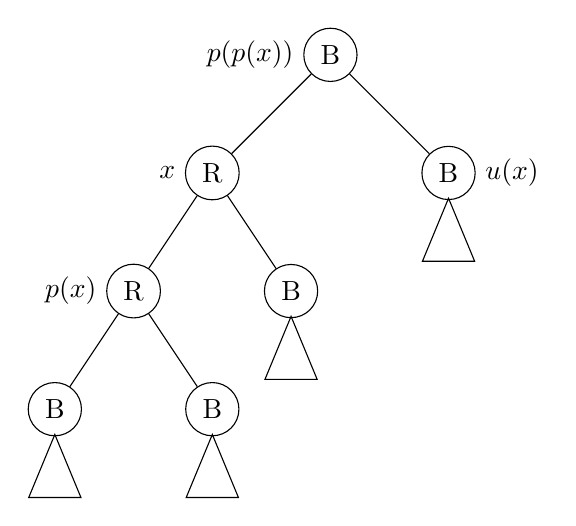
\begin{tikzpicture}[sibling distance=3cm, level 2/.style={sibling distance
	=2cm}]
	\node[draw, circle, label=west:$p(p(x))$] {B}
	child{ node[circle, draw, label=west:$x$] {R} 
		child { node[circle, draw, label=west:$p(x)$] {R}
			child { node[circle, draw] {B} { node[subtree] {} }}
			child { node[circle, draw] {B} { node[subtree] {} }}
		}
		child { node[circle, draw] {B} { node[subtree] {} }}
	}
	child{ node[circle, draw, label=east:$u(x)$] {B} { node[subtree] {} }};
\end{tikzpicture}
\end{center}
In this case we perform a left rotate of $p(x)$. and we are back the earlier
case ($x$ being left child of $p(x)$) with the only difference that $p(x)$
will be the new $x$ (Comparing the figures in this case and the previous one
helps). 

{\bf Sub case 2 -- $p(x)$ is the right child of $p(p(x))$ :} The situation is
as shown. Here we need to perform a right rotate of $p(x)$. After the
rotation, it can be seen that all $x$, $p(x)$ and $p(p(x))$ are right child of
their parents.  
\begin{center}
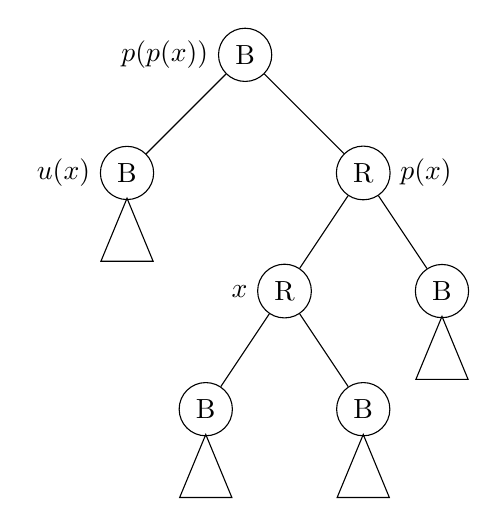
\begin{tikzpicture}[sibling distance=3cm, level 2/.style={sibling distance
	=2cm}]
	\node[draw, circle, label=west:$p(p(x))$] {B}
	child{ node[circle, draw, label=west:$u(x)$] {B} { node[subtree] {} }}
	child{ node[circle, draw, label=east:$p(x)$] {R} 
		child { node[circle, draw, label=west:$x$] {R}
			child { node[circle, draw] {B} { node[subtree] {} }}
			child { node[circle, draw] {B} { node[subtree] {} }}
		}
		child { node[circle, draw] {B} { node[subtree] {} }}
	};
\end{tikzpicture} \quad\quad
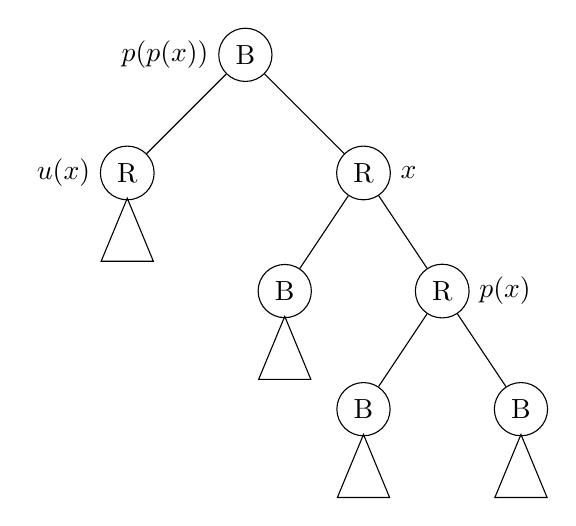
\begin{tikzpicture}[sibling distance=3cm, level 2/.style={sibling distance
	=2cm}]
	\node[draw, circle, label=west:$p(p(x))$] {B}
	child{ node[circle, draw, label=west:$u(x)$] {R} { node[subtree] {} }}
	child{ node[circle, draw, label=east:$x$] {R} 
		child { node[circle, draw] {B} { node[subtree] {} }}
		child { node[circle, draw, label=east:$p(x)$] {R}
			child { node[circle, draw] {B} { node[subtree] {} }}
			child { node[circle, draw] {B} { node[subtree] {} }}
		}
	};
\end{tikzpicture}
\end{center}
Note that this is a mirror reflection of the case where all of them were left
child. So a symmetric set of operations can be done for this case. {\em 
The set of operations required are outlined for the sake of completeness.}

Similar to the case where $x$ is left child of $p(x)$, first we interchange
the colors of $p(x)$ and $p(p(x))$ and get the following. 

\begin{center}
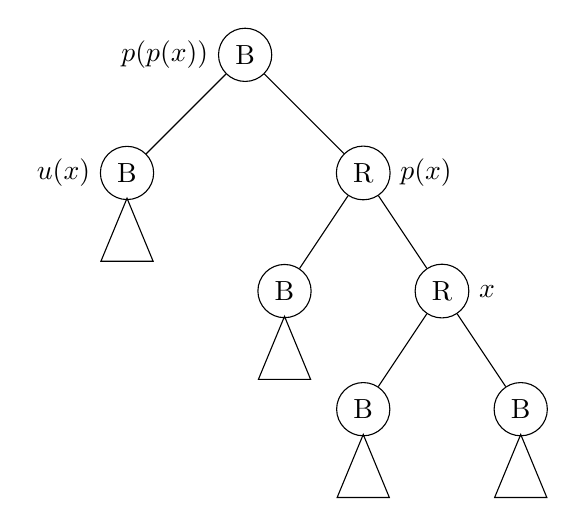
\begin{tikzpicture}[sibling distance=3cm, level 2/.style={sibling distance
	=2cm}]
	\node[draw, circle, label=west:$p(p(x))$] {B}
	child{ node[circle, draw, label=west:$u(x)$] {B} { node[subtree] {} }}
	child{ node[circle, draw, label=east:$p(x)$] {R} 
		child { node[circle, draw] {B} { node[subtree] {} }}
		child { node[circle, draw, label=east:$x$] {R}
			child { node[circle, draw] {B} { node[subtree] {} }}
			child { node[circle, draw] {B} { node[subtree] {} }}
		}
	};
\end{tikzpicture} 
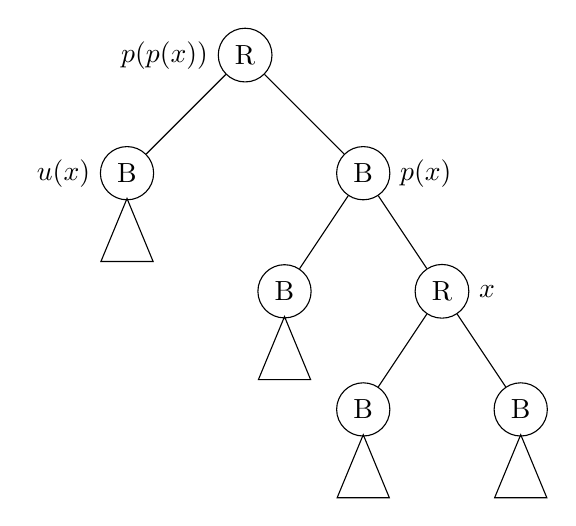
\begin{tikzpicture}[sibling distance=3cm, level 2/.style={sibling distance
	=2cm}]
	\node[draw, circle, label=west:$p(p(x))$] {R}
	child{ node[circle, draw, label=west:$u(x)$] {B} { node[subtree] {} }}
	child{ node[circle, draw, label=east:$p(x)$] {B} 
		child { node[circle, draw] {B} { node[subtree] {} }}
		child { node[circle, draw, label=east:$x$] {R}
			child { node[circle, draw] {B} { node[subtree] {} }}
			child { node[circle, draw] {B} { node[subtree] {} }}
		}
	};

\end{tikzpicture}
\end{center}

With this interchange, black height along the left child of
$p(p(x))$ has increased by $1$ while along the right remained the same. So to
balance out, we perform a rotation of $p(p(x))$ around $p(x)$ (i,e. left 
rotate of $p(p(x))$).

\begin{center}
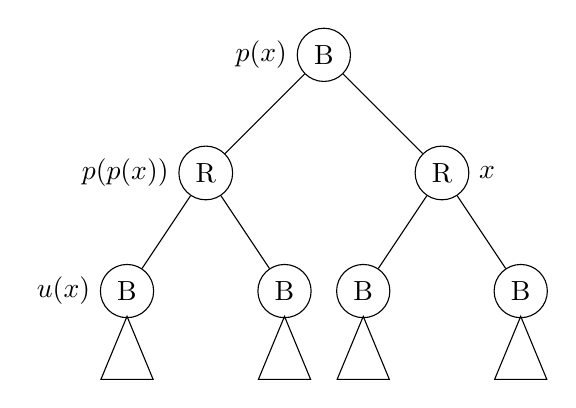
\begin{tikzpicture}[sibling distance=3cm, level 2/.style={sibling distance
	=2cm}]
	\node[draw, circle, label=west:$p(x)$] {B}
	child{ node[circle, draw, label=west:$p(p(x))$] {R} 
		child { node[circle, draw, label=west:$u(x)$] {B} { node[subtree] {} }}
		child { node[circle, draw] {B} { node[subtree] {} }}
	}
	child{ node[circle, draw, label=east:$x$] {R} 
		child { node[circle, draw] {B} { node[subtree] {} }}
		child { node[circle, draw] {B} { node[subtree] {} }}
	};
\end{tikzpicture}
\end{center}
Now note that there is no more red-red violation and right rotation re-balances
the black height. Since there are no more violations we can stop here. Note
that the outcomes are also very symmetric when compared to the previous case. 

Pseudo code corresponding to reducing the case of
node being a right child to node being a left child of parent and its symmetric
case is given below.

\begin{verbatim}
fixup-Uncle-black-spl(Node* node)
{
        Node* gp = grandparent(node);
        if(node == node->parent->right && node->parent == gp->left){
                left_rotate(node->parent);
                node = node->left;
        }else if(node == node->parent->left && node->parent == gp->right){
                right_rotate(node->parent);
                node = node->right;
        }
        fixup-Uncle-Black(node);
}
\end{verbatim}

Pseudo code corresponding to fixing the violation is as shown.
\begin{verbatim}
fixup-Uncle-Black(Node* node)
{
        Node* gp = grandparent(node);
        node->parent->colour = BLACK;
        gp->colour = RED;

        if(node == node->parent->left && node->parent == gp->left)
                right_rotate(gp);
        else if(node == node->parent->right && node->parent == gp->right)
                left_rotate(gp);
        return 0; // Halt
}

\end{verbatim}

\subsection{Main Idea in Deletion}
In binary search tree deletion of a node, we finally arrive at a case where
the node to be deleted has at most one child. But in a RB tree there is
always a black sentinel node attached to every leaf. So to be precise,
we reach a non-sentinel child. Let $x$ be the node to be deleted. Following are the major two cases which happens.
\begin{enumerate}
	\item Leaf node to be deleted has exactly one non-sentinel child.
	\item Leaf node to be deleted has both sentinel children.
\end{enumerate}

\fbox{{\bf Node to be deleted has exactly one non sentinel child :}}
Let $c(x)$ denote the only child of $x$. In the first case, we can have four
sub cases based on the color of $x$ and $c(x)$. 

\begin{center}
	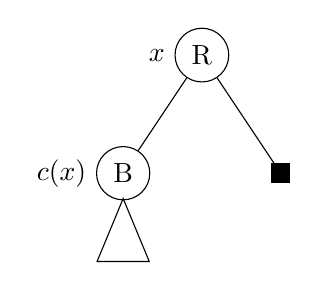
\begin{tikzpicture}[sibling distance=2cm]
		\node[draw,circle,label=west:$x$] {R}
		child{ node[draw, circle, label=west:$c(x)$] {B}
		{node[subtree] {}}} 
		child{ node[draw, rectangle, fill=black] {} };
	\end{tikzpicture}\quad
	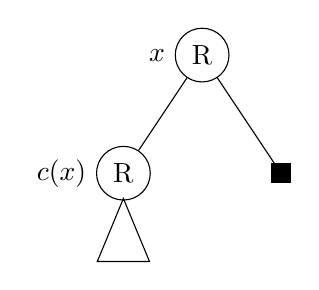
\begin{tikzpicture}[sibling distance=2cm]
		\node[draw,circle,label=west:$x$] {R}
		child{ node[draw, circle, label=west:$c(x)$] {R}
		{node[subtree] {}} }
		child{ node[draw, rectangle, fill=black] {} };
	\end{tikzpicture}\quad
	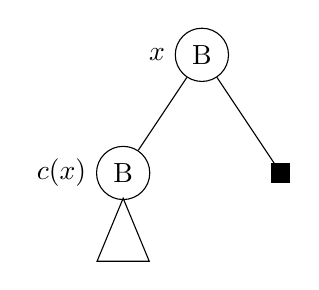
\begin{tikzpicture}[sibling distance=2cm]
		\node[draw,circle,label=west:$x$] {B}
		child{ node[draw, circle, label=west:$c(x)$] {B}
		{node[subtree] {}} }
		child{ node[draw, rectangle, fill=black] {} };
	\end{tikzpicture}\quad
	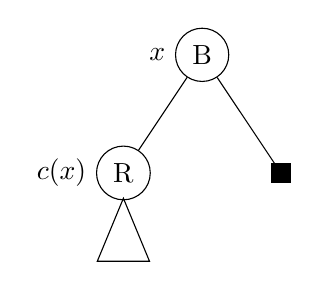
\begin{tikzpicture}[sibling distance=2cm]
		\node[draw,circle,label=west:$x$] {B}
		child{ node[draw, circle, label=west:$c(x)$] {R}
		{node[subtree] {}} }
		child{ node[draw, rectangle, fill=black] {}};
	\end{tikzpicture}
\end{center}

Note that the first three sub cases are not possible as there is black height
violation, red-red violation and black height violation
respectively. The last case is possible and can be handled in the following
way.  
\begin{itemize}
	\item If $x$ has no parent, $x$ must be the root. We can simply
		make $c(x)$ as the new root and color it black and remove $x$. 
		All properties are satisfied. 
	\item If $x$ has a parent, make parent of $x$ same as parent of $c(x)$
		and color $c(x)$ black and remove $x$. Here, recoloring
		ensures that root is black and there are no more violations.
\end{itemize}
In both cases there are no more violations and we can halt.

\fbox{{\bf Node to be deleted has both sentinels :}}
Here again there are two cases where the leaf node is a red or black.
In the case where node is red, we can directly delete the node as this does not
violate any of the properties.  The case where {\bf node is black and both
children are sentinels} is the only case left to be handled. We explain how to
handle this case in the subsequent sections.

\subsection{Fixing the violation in RB-tree after Tree deletion} 
The case that we need to handle now has the node to be deleted (which is $x$)
being a black leaf node with children being sentinels. 

For generality of argument, we shall consider left child of $x$ to be a
subtree. Note that it can also be an empty subtree in which case it is a
sentinel. We will see later where exactly this assumption helps. Note that
all arguments outlined henceforth will hold irrespective of what the left child
of $x$ is. Color of $c(x)$ is black as we have already dealt with the case when 
$c(x)$ is red.
\begin{center}
	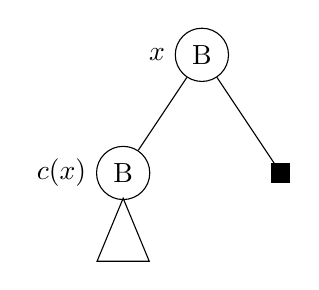
\begin{tikzpicture}[sibling distance=2cm]
		\node[draw,circle,label=west:$x$] {B}
		child{ node[draw, circle, label=west:$c(x)$] {B}
		{node[subtree] {}}} 
		child{ node[draw, rectangle, fill=black] {} };
	\end{tikzpicture}
\end{center}
Here we have two cases based on whether $x$ has a parent or not. If $x$ has no
parent, then $x$ must be the root and we can simply make $c(x)$ as the new
root and delete $x$.

If $x$ has a parent, we have the following situation. 
\begin{center}
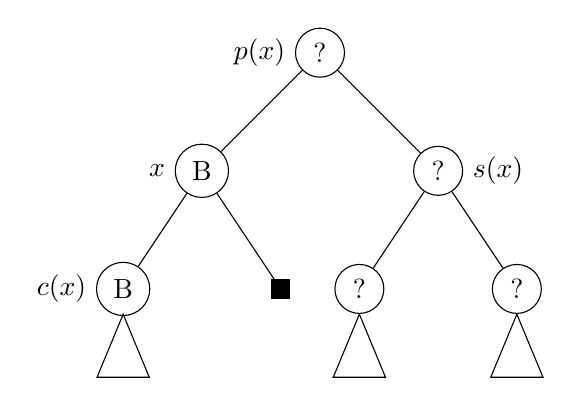
\begin{tikzpicture}[sibling distance=3cm, level 2/.style={sibling distance
	=2cm}]
	\node[draw, circle, label=west:$p(x)$] {?}
	child{ node[circle, draw, label=west:$x$] {B} 
		child { node[circle, draw, label=west:$c(x)$] {B} { node[subtree] {} }}
		child{ node[draw, rectangle, fill=black] {} }
	}
	child{ node[circle, draw, label=east:$s(x)$] {?} 
		child { node[circle, draw] {?} { node[subtree] {} }}
		child { node[circle, draw] {?} { node[subtree] {} }}
	};
\end{tikzpicture}\quad
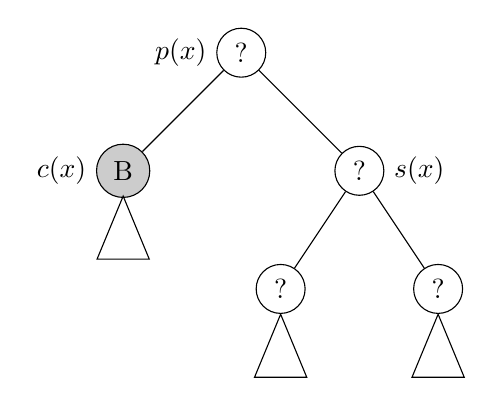
\begin{tikzpicture}[sibling distance=3cm, level 2/.style={sibling distance
	=2cm}]
	\node[draw, circle, label=west:$p(x)$] {?}
	child { node[circle,fill=black!20, draw, label=west:$c(x)$] {B} { node[subtree] {} }}
	child{ node[circle, draw, label=east:$s(x)$] {?} 
		child { node[circle, draw] {?} { node[subtree] {} }}
		child { node[circle, draw] {?} { node[subtree] {} }}
	};
\end{tikzpicture}\quad
\end{center}
Here we assume that \emph{$x$ is the left child of $p(x)$}\footnote{A
	symmetric set of operations would work in the case when $x$ is a right
child.}. We explain briefly why do we have the following structure. Call the
right child of $p(x)$ as \emph{sibling} of $x$ (denoted as $s(x)$). 

Note that $s(x)$ cannot be a sentinel node, for otherwise the black height
along left path starting from $p(x)$ will be at least $2$ while along the
right path will be only $1$. Since $s(x)$ is not a sentinel, we can always
speak of its children (which may be sentinels). The question marks corresponds
to the colors of the nodes which are currently not inferable.

In this case, we delete node $x$ and make $c(x)$ as child of $p(x)$ (picture
on right). The black color of $x$ is given to $c(x)$ making it \emph{doubly
black} (shown in shaded). Now that we have deleted $x$, in the rest of the
cases that arise, our aim is to get rid of the this double blackness. Note
that all properties are satisfied except that $c(x)$ is doubly black. Hence
while handling each of the cases we can assume this. 

Even though there are $4$ unknown colors which
could potentially lead to $16$ sub cases, we will show how we can tackle many
cases at one shot.  There are two main cases, one where sibling of $x$ is
black and other where sibling of $x$ is red. 
\subsubsection{Sibling is black}
Here there can three exhaustive sub cases which are as follows.
\begin{enumerate}
	\item Left and right child of $s(x)$ are black
	\item Right child of $s(x)$ is red
	\item Left child of $s(x)$ is red and right child of $s(x)$ is black
\end{enumerate}

\fbox{{\bf Left and right child of $s(x)$ are black}}
\begin{center}
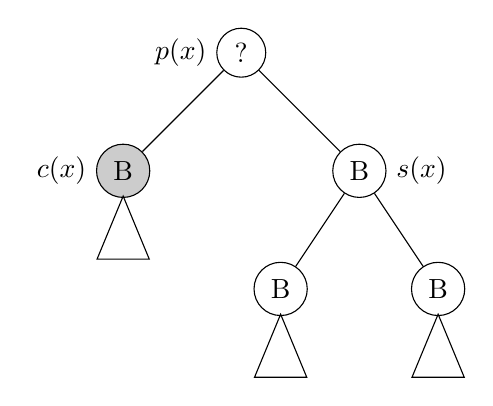
\begin{tikzpicture}[sibling distance=3cm, level 2/.style={sibling distance
	=2cm}]
	\node[draw, circle, label=west:$p(x)$] {?}
	child { node[circle,fill=black!20, draw, label=west:$c(x)$] {B} { node[subtree] {} }}
	child{ node[circle, draw, label=east:$s(x)$] {B} 
		child { node[circle, draw] {B} { node[subtree] {} }}
		child { node[circle, draw] {B} { node[subtree] {} }}
	};
\end{tikzpicture}
\end{center}
From the figure, we can see that there can be two sub cases one where $p(x)$ is
red and one where $p(x)$ is black. 
In both cases, we ``pull'' one black from the left and right of $p(x)$ leaving
$c(x)$ with one black and making $s(x)$ red. If $p(x)$ is red, we color it
black and there are no extra violations. If $p(x)$ is black, the extra black
color will reach $p(x)$ and we need to recursively invoke the whole deletion 
procedure (only the non-base cases) with $p(x)$ as the new $x$.

Also since the children of $s(x)$ are already black, coloring $s(x)$ to red
will not create any violation. Figure shows both the cases in action.

{\bf Sub case 1 -- $p(x)$ is red :} 
\begin{center}
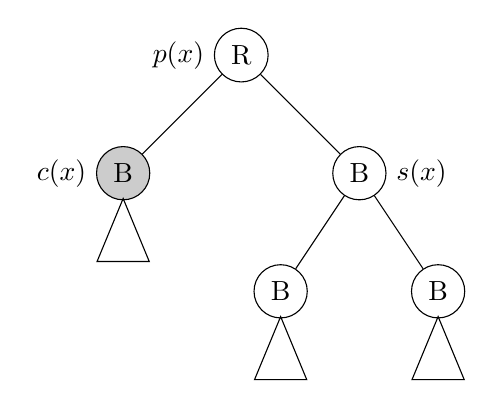
\begin{tikzpicture}[sibling distance=3cm, level 2/.style={sibling distance
	=2cm}]
	\node[draw, circle, label=west:$p(x)$] {R}
	child { node[circle,fill=black!20, draw, label=west:$c(x)$] {B} { node[subtree] {} }}
	child{ node[circle, draw, label=east:$s(x)$] {B} 
		child { node[circle, draw] {B} { node[subtree] {} }}
		child { node[circle, draw] {B} { node[subtree] {} }}
	};
\end{tikzpicture} \quad
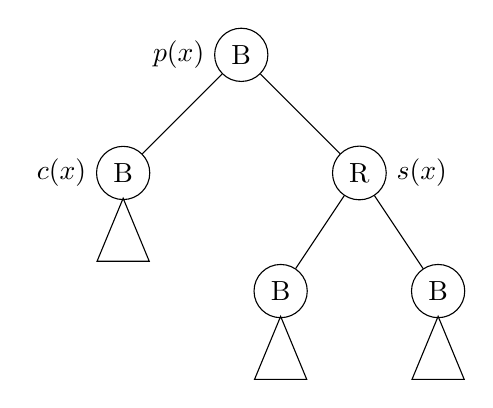
\begin{tikzpicture}[sibling distance=3cm, level 2/.style={sibling distance
	=2cm}]
	\node[draw, circle, label=west:$p(x)$] {B}
	child { node[circle, draw, label=west:$c(x)$] {B} { node[subtree] {} }}
	child{ node[circle, draw, label=east:$s(x)$] {R} 
		child { node[circle, draw] {B} { node[subtree] {} }}
		child { node[circle, draw] {B} { node[subtree] {} }}
	};
\end{tikzpicture}
\end{center}

{\bf Sub case 2 -- $p(x)$ is black :}
\begin{center}
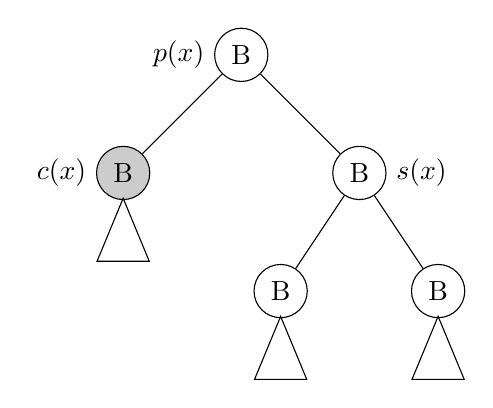
\begin{tikzpicture}[sibling distance=3cm, level 2/.style={sibling distance
	=2cm}]
	\node[draw, circle, label=west:$p(x)$] {B}
	child { node[circle,fill=black!20, draw, label=west:$c(x)$] {B} { node[subtree] {} }}
	child{ node[circle, draw, label=east:$s(x)$] {B} 
		child { node[circle, draw] {B} { node[subtree] {} }}
		child { node[circle, draw] {B} { node[subtree] {} }}
	};
\end{tikzpicture} \quad
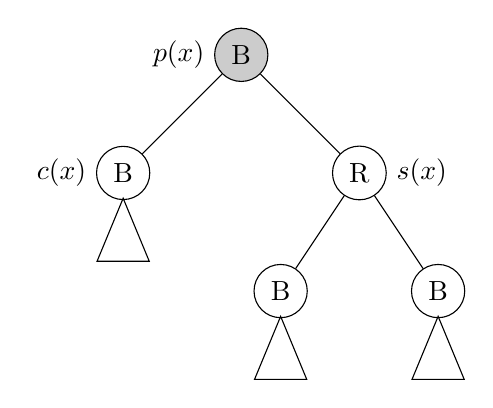
\begin{tikzpicture}[sibling distance=3cm, level 2/.style={sibling distance
	=2cm}]
	\node[draw, circle, ,fill=black!20,label=west:$p(x)$] {B}
	child { node[circle, draw, label=west:$c(x)$] {B} { node[subtree] {} }}
	child{ node[circle, draw, label=east:$s(x)$] {R} 
		child { node[circle, draw] {B} { node[subtree] {} }}
		child { node[circle, draw] {B} { node[subtree] {} }}
	};
\end{tikzpicture}
\end{center}

\fbox{{\bf Right child of $s(x)$ is red}}
Let color of $p(x)$ be $X$ and color of left child of $s(x)$ be $Y$ where
$X,Y$ can be any of red or black. 
\begin{center}
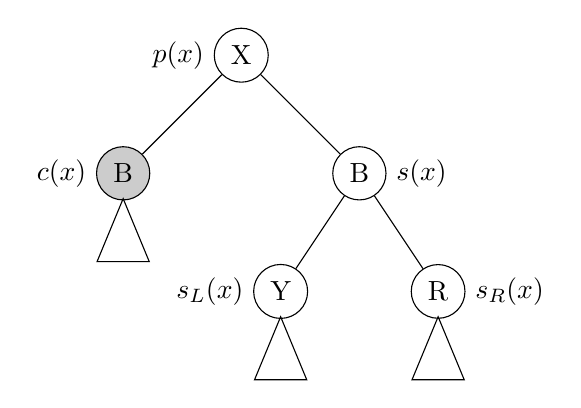
\begin{tikzpicture}[sibling distance=3cm, level 2/.style={sibling distance
	=2cm}]
	\node[draw, circle, label=west:$p(x)$] (top) {X}
	child { node[circle,fill=black!20, draw, label=west:$c(x)$]  {B} { node[subtree] {} }}
	child{ node[circle, draw, label=east:$s(x)$] {B} 
		child { node[circle, draw, label=west:$s_L(x)$] {Y} { node[subtree] {} }}
		child { node[circle, draw, label=east:$s_R(x)$] {R} { node[subtree] {} }}
	};
\end{tikzpicture} \quad
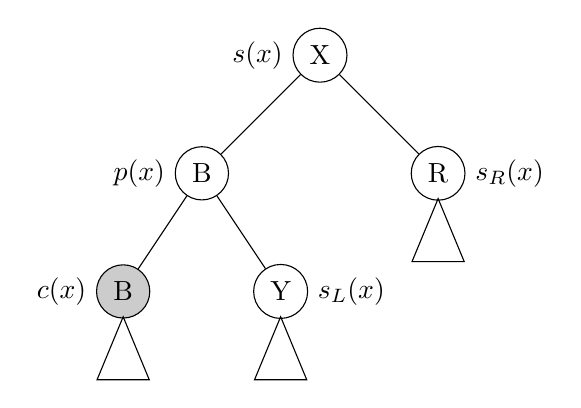
\begin{tikzpicture}[sibling distance=3cm, level 2/.style={sibling distance
	=2cm}]
	\node[draw, circle, label=west:$s(x)$] {X}
	child{ node[circle, draw, label=west:$p(x)$] {B} 
		child { node[circle, draw, fill=black!20, label=west:$c(x)$] {B} { node[subtree] {} }}
		child { node[circle, draw, label=east:$s_L(x)$] {Y} { node[subtree] {} }}
	}
	child { node[circle, draw, label=east:$s_R(x)$] {R} { node[subtree] {} }};
\end{tikzpicture}
\end{center}

We perform the following.
\begin{enumerate}
	\item Interchange the colors of $p(x)$ and $s(x)$ and do a left 
		rotate of $p(x)$. 
	\item Color the right child of $s(x)$ (which was red) black.
\end{enumerate}
In the figure, we have shown only the first step.

Let us now see what has happened to the black heights of the nodes. Let $bh+1$
be the black height of $p(x)$\footnote{Recall that black height of a
non-sentinel node is at least $1$} where $bh \ge 0$.  We now argue that for
any color for $X, Y$ the black height of $s(x)$ will be $bh+1$ after the
transformation.

Firstly observe that before the transformation, since black height of $p(x)$
is $bh+1$, black height of $c(x)$ is $bh-1$ (obtained from $bh+1 - 2$), black
height of $s(x)$, $s_R(x)$ is $bh$ (obtained from $bh+1 - 1$). After the transformation,
\begin{itemize}
	\item along the path $s(x)$ --- $p(x)$ --- $c(x)$, the black height is
		$bh - 1+2+1 = bh+2$. 
	\item along the path $s(x)$ --- $p(x)$ --- $s_L(x)$, note that the color
		of the nodes along this path is the same as that of the path
		$s(x)$ --- $s_L(x)$ before the transformation and hence 
		the black height should remains the same as $bh+1$.
	\item along the path $s(x)$ --- $s_R(x)$, the black height is $bh$.
\end{itemize}

Note that there is a clear imbalance of black heights. Now comes the
significance of the second step. Coloring $s_R(x)$ black increase
black height along $s(x)$ --- $s_R(x)$ to $bh+1$. We can see this coloring as
``using up'' of the extra blackness of $c(x)$. With this, black height along
$s(x)$ --- $p(x)$ --- $c(x)$ get reduced to $bh+1$. Final outcome is as shown.
It can be seen that there are no more violations. 
\begin{center}
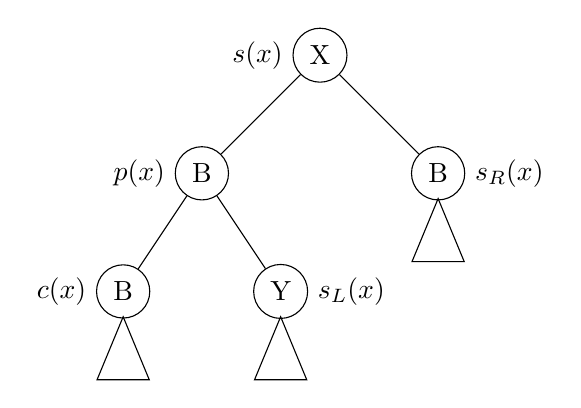
\begin{tikzpicture}[sibling distance=3cm, level 2/.style={sibling distance
	=2cm}]
	\node[draw, circle, label=west:$s(x)$] {X}
	child{ node[circle, draw, label=west:$p(x)$] {B} 
		child { node[circle, draw, label=west:$c(x)$] {B} { node[subtree] {} }}
		child { node[circle, draw, label=east:$s_L(x)$] {Y} { node[subtree] {} }}
	}
	child { node[circle, draw, label=east:$s_R(x)$] {B} { node[subtree] {} }};
\end{tikzpicture}
\end{center}

Note that we have not used any information regarding what $X, Y$ are and hence
this argument work for any $X, Y$. Hence in particular the cases with right
child of $s(x)$ is red, left child being red/black are covered. We have
already covered the case where right and left children are black (which was
our first case). So we are left the only case where right child is black and
left child is red.

\fbox{{\bf Left child of $s(x)$ is red and right child of $s(x)$ is black}}
The situation is as shown. We do not know the color of $p(x)$. The argument
however works irrespective of its color.
\begin{center}
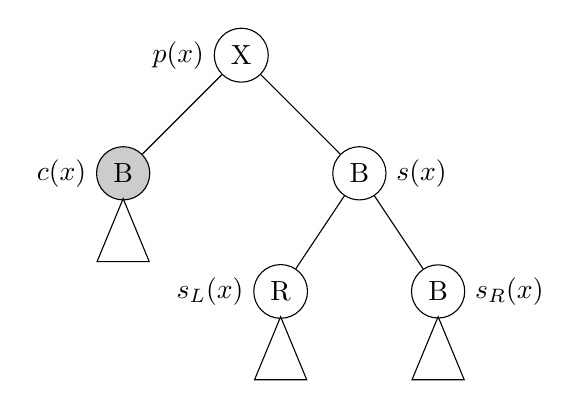
\begin{tikzpicture}[sibling distance=3cm, level 2/.style={sibling distance
	=2cm}]
	\node[draw, circle, label=west:$p(x)$] (top) {X}
	child { node[circle,fill=black!20, draw, label=west:$c(x)$] {B} { node[subtree] {} }}
	child{ node[circle, draw, label=east:$s(x)$] {B} 
		child { node[circle, draw, label=west:$s_L(x)$] {R} { node[subtree] {} }}
		child { node[circle, draw, label=east:$s_R(x)$] {B} { node[subtree] {} }}
	};
\end{tikzpicture}
\end{center}
This case can be reduced to the previous case : ``the right child of $s(x)$
is red'' by the following observation.  Since $s_L(x)$ is red, it must be that
both its children are black.
\begin{center}
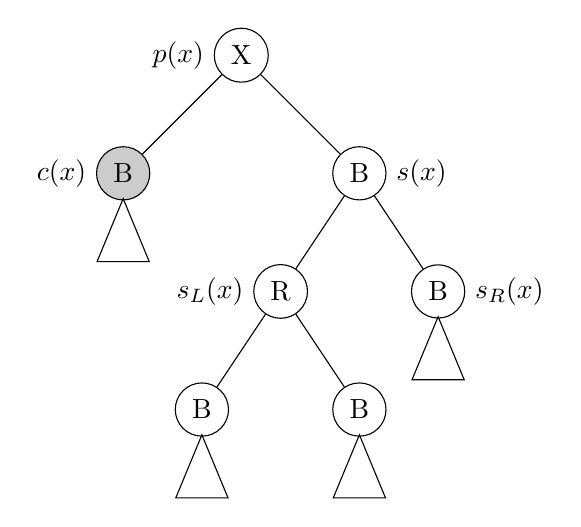
\begin{tikzpicture}[sibling distance=3cm, level 2/.style={sibling distance
	=2cm}]
	\node[draw, circle, label=west:$p(x)$] {X}
	child { node[circle,fill=black!20, draw, label=west:$c(x)$] {B} { node[subtree] {} }}
	child{ node[circle, draw, label=east:$s(x)$] {B} 
		child { node[circle, draw, label=west:$s_L(x)$] {R} 
			child{ node[circle, draw] {B} { node[subtree] {} }}
			child{ node[draw, circle] {B} { node[subtree] {} }}
		}
		child { node[circle, draw, label=east:$s_R(x)$] {B} { node[subtree] {} }}
	};
\end{tikzpicture} \quad
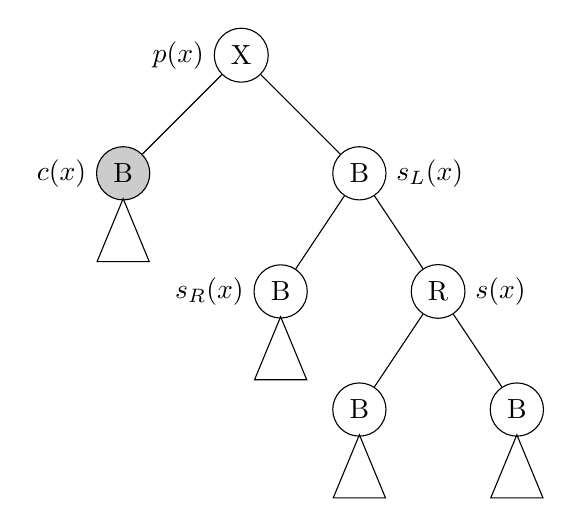
\begin{tikzpicture}[sibling distance=3cm, level 2/.style={sibling distance
	=2cm}]
	\node[draw, circle, label=west:$p(x)$] {X}
	child { node[circle,fill=black!20, draw, label=west:$c(x)$] {B} { node[subtree] {} }}
	child{ node[circle, draw, label=east:$s_L(x)$] {B} 
		child { node[circle, draw, label=west:$s_R(x)$] {B} { node[subtree] {} }}
		child { node[circle, draw, label=east:$s(x)$] {R} 
			child{ node[circle, draw] {B} { node[subtree] {} }}
			child{ node[draw, circle] {B} { node[subtree] {} }}
		}
	};
\end{tikzpicture}
\end{center}
Our aim is to come with a transformation such that the right child of $s(x)$
is red.  This can be achieved if we swap the color of $s_L(x)$ and $s(x)$ and
right rotate $s(x)$. Moreover swapping of colors compensate for the reduction
in black height of $s_L(x)$ due to rotation. After the transformation, we can
treat the $s_L(x)$ as our new $s(x)$ (see figure on right) and run the case
 ``right child of s(x) is red'' to handle this case.

\subsubsection{Sibling is red}
The situation is as shown. Since $s(x)$ is red, both its parent and children
must be black.
\begin{center}
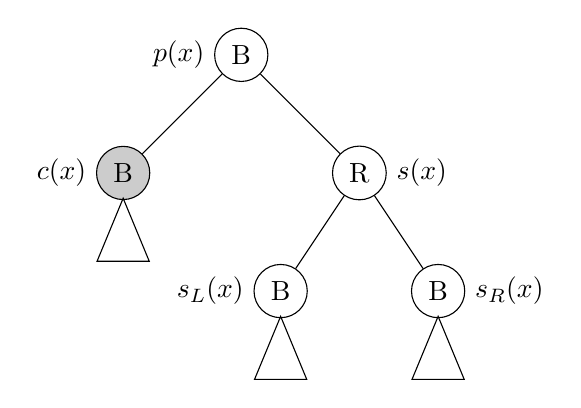
\begin{tikzpicture}[sibling distance=3cm, level 2/.style={sibling distance
	=2cm}]
	\node[draw, circle, label=west:$p(x)$]  {B}
	child { node[circle,fill=black!20, draw, label=west:$c(x)$] {B} { node[subtree] {} }}
	child{ node[circle, draw, label=east:$s(x)$] {R} 
		child { node[circle, draw, label=west:$s_L(x)$] {B} { node[subtree] {} }}
		child { node[circle, draw, label=east:$s_R(x)$] {B} { node[subtree] {} }}
	};
\end{tikzpicture} \quad
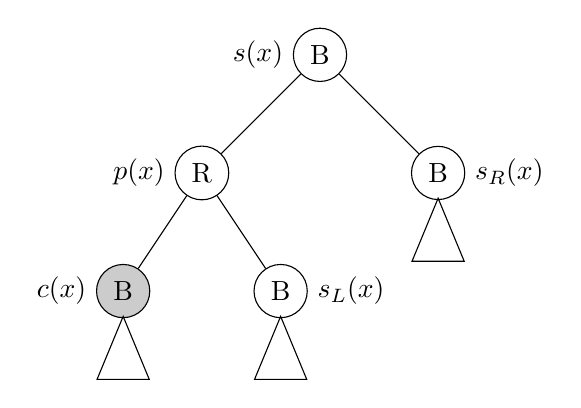
\begin{tikzpicture}[sibling distance=3cm, level 2/.style={sibling distance
	=2cm}]
	\node[draw, circle, label=west:$s(x)$]  {B}
	child{ node[circle, draw, label=west:$p(x)$] {R} 
		child { node[circle, draw, fill=black!20,label=west:$c(x)$] {B} { node[subtree] {} }}
		child { node[circle, draw, label=east:$s_L(x)$] {B} { node[subtree] {} }}
	}
	child { node[circle, draw, label=east:$s_R(x)$] {B} {
	node[subtree] {} }};
\end{tikzpicture}
\end{center}
In this case, we can left rotate $p(x)$ and to compensate for the black height
reduction, interchange the colors of $s(x), p(x)$ before rotation. After the
transformation note that the right child of $s(x)$, is black. So we treat
$s_R(x)$ as the sibling of $x$ and it black in color thereby we fall to the
case ``sibling is black''. By going through the appropriate cases the
violation is removed. Also note that since our main two cases are disjoint
there cannot be an infinite recursion.
\end{document}
